%%%%%%%%%%%%%%%%%%%%%%%%%%%%%%%%%%%%%%%%%%%%%%%%%%%%%%%%%%%%%%%
%
% Welcome to Overleaf --- just edit your LaTeX on the left,
% and we'll compile it for you on the right. If you open the
% 'Share' menu, you can invite other users to edit at the same
% time. See www.overleaf.com/learn for more info. Enjoy!
%
%%%%%%%%%%%%%%%%%%%%%%%%%%%%%%%%%%%%%%%%%%%%%%%%%%%%%%%%%%%%%%%

% ===============================================
% MATH 790: Real Analysis           Spring 2022
% hw_template.tex
% ===============================================

% -------------------------------------------------------------------------
% The preamble that follows can be ignored. Go on
% down to the section that says "START HERE" 
% -------------------------------------------------------------------------

\documentclass{article}

\usepackage[margin=1in]{geometry} 
\usepackage{amsmath,amsthm,amssymb,hyperref,graphicx}
\usepackage[hangul]{kotex}
\usepackage[shortlabels]{enumitem}
\usepackage{booktabs, multicol, multirow} % Allows the use of \toprule, \midrule and \bottomrule in tables

\newcommand{\R}{\mathbf{R}}  
\newcommand{\Z}{\mathbf{Z}}
\newcommand{\N}{\mathbf{N}}
\newcommand{\Q}{\mathbf{Q}}

\renewcommand{\labelenumii}{\arabic{enumi}.\arabic{enumii}}
\renewcommand{\labelenumiii}{\arabic{enumi}.\arabic{enumii}.\arabic{enumiii}}
\renewcommand{\labelenumiv}{\arabic{enumi}.\arabic{enumii}.\arabic{enumiii}.\arabic{enumiv}}

\newenvironment{theorem}[2][Theorem]{\begin{trivlist}
\item[\hskip \labelsep {\bfseries #1}\hskip \labelsep {\bfseries #2.}]}{\end{trivlist}}
\newenvironment{lemma}[2][Lemma]{\begin{trivlist}
\item[\hskip \labelsep {\bfseries #1}\hskip \labelsep {\bfseries #2.}]}{\end{trivlist}}
\newenvironment{exercise}[2][Exercise]{\begin{trivlist}
\item[\hskip \labelsep {\bfseries #1}\hskip \labelsep {\bfseries #2.}]}{\end{trivlist}}
\newenvironment{problem}[2][Problem]{\begin{trivlist}
\item[\hskip \labelsep {\bfseries #1}\hskip \labelsep {\bfseries #2.}]}{\end{trivlist}}
\newenvironment{question}[2][Question]{\begin{trivlist}
\item[\hskip \labelsep {\bfseries #1}\hskip \labelsep {\bfseries #2.}]}{\end{trivlist}}
\newenvironment{corollary}[2][Corollary]{\begin{trivlist}
\item[\hskip \labelsep {\bfseries #1}\hskip \labelsep {\bfseries #2.}]}{\end{trivlist}}

\newenvironment{solution}{\begin{proof}[Solution]}{\end{proof}}

\begin{document}

% ------------------------------------------ %
%                 START HERE                  %
% ------------------------------------------ %

\title{경제정의와 불평등 기말고사} % Replace with appropriate title
\author{담당교수 : 오성재} % Replace "Author's Name" with your name
\date{\today}

\maketitle

% -----------------------------------------------------
% The following two environments (theorem, proof) are
% where you will enter the statement and proof of your
% first problem for this assignment.
%
% In the theorem environment, you can replace the word
% "theorem" in the \begin and \end commands with
% "exercise", "problem", "lemma", etc., depending on
% what you are submitting. 
% -----------------------------------------------------
\begin{enumerate}[{\bf 문제 \arabic*.}]
    
    \item 그림\ref{simpled}은 3인으로 구성된 사회에서 실현가능한 서로 다른 분배상태 $1,2,3$을 나타내고 있다.
        \begin{figure}[htbp]
            \centering
            \caption{간단한 소득분포}
            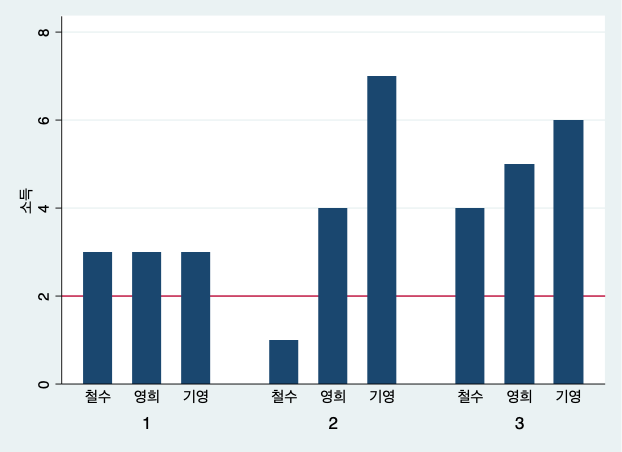
\includegraphics[width=0.5\textwidth]{pic/simpledist.png}
            \label{simpled}
        \end{figure}
        \begin{enumerate}
            \item 효용의 원칙을 정의하시오. 어떤 분배상태가 이 원칙을 가장 잘 구현하는지 설명하시오.
            \item 평등의 원칙을 정의하시오. 어떤 분배상태가 이 원칙을 가장 잘 구현하는지 설명하시오.
            \item 충분성의 원칙을 정의하시오. 소득 2가 충분성의 기준일 때, 각각의 분배상태가 이를 만족하는 지의 여부를 설명하시오.
            \item 우선의 원칙을 정의하시오. 영희가 선천적 장애를 타고 났다면 어떤 분배상태가 우선의 원칙을 가장 잘 구현하는지 설명하시오.
        \end{enumerate}

    \item 우파적 자유주의의 정의관을 엄밀하게 정의하시오. 이를 구현하기 위한 사회적 장치에 대하여 약술 하시오.
    
    \item 좌파적 자유주의의 정의관을 엄밀하게 정의하시오. 이들이 생각하는 이상적인 사회장치에 대하여 약술 하시오.
    
    \item 좌파적 자유주의가 생각하는 인간관과 이를 위한 특성을 서술하시오. 또한 우파적 자유주의의 인간관과 어떻게 다른지 약술하시오.
    
\pagebreak
    
    \item 효율적인 분배의 판단기준을 엄밀하게 정의하시오.

    \item 그림 \ref{pe}는 a,b 두 사람으로 구성된 사회에서 실현가능한 효용의 분배를 효용가능경계를 통해 나타낸 것이다.
        \begin{figure}[htbp]
            \centering
            \caption{다양한 분포들}
            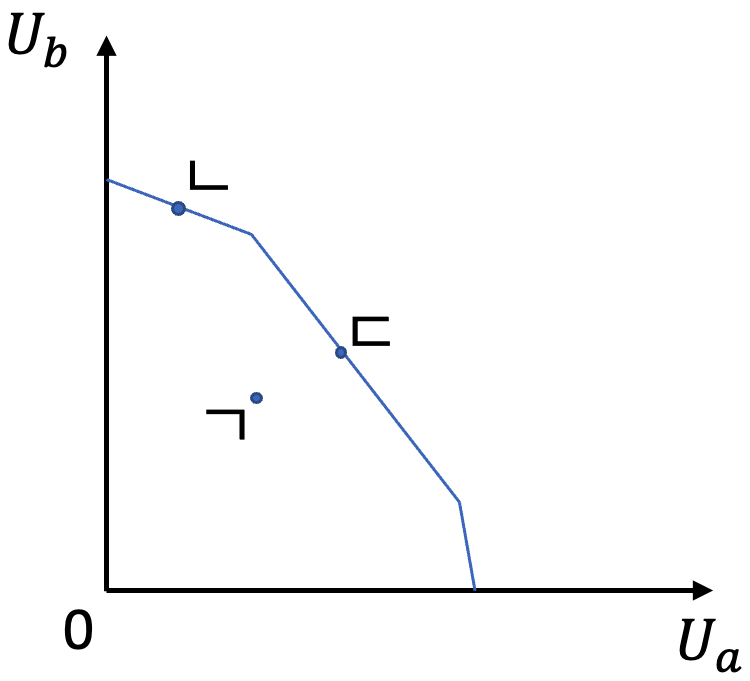
\includegraphics[width=0.5\textwidth]{pic/ParetoE.png}
            \label{pe}
        \end{figure}
        \begin{enumerate}
            \item 분배 ㄱ은 효율적인 분배인지 여부를 판단하고 근거를 약술하시오.
            \item 분배 ㄴ과 ㄷ 가운데 어느것이 더 효율적인 분배인지 판단하고 근거를 약술하시오.
        \end{enumerate}
    

    \item 후생경제학 제 1정리와 제 2정리에 대하여 엄밀히 정의하고, 그 의미를 약술하시오.
    
    \item 사회후생함수의 존재를 가정하자. 효용가능경계는 그림\ref{pe}와 같은 형태로 주어진다.
        \begin{enumerate}
            \item 사회가 공리주의적 미덕을 가질때 최적의 분배를 그림을 통해 설명하시오.
            \item 사회가 우파적 자유주의의 미덕을 가질때 최적의 분배를 그림을 통해 설명하시오.
            \item 사회가 좌파적 자유주의의 미덕을 가질때 최적의 분배를 그림을 통해 설명하시오.
        \end{enumerate}
        
    \item 사회후생함수에 대한 불가능성 정리를 엄밀히 정의하고, 그 의미를 약술하시오.

\vspace{3cm}

    \centering
    \large{중간고사 고생하셨습니다.}
  
\end{enumerate}



% ---------------------------------------------------
% Anything after the \end{document} will be ignored by the typesetting.
% ----------------------------------------------------

\end{document}